% Capítulo 4
\chapter{A matemática dos movimentos}
\label{ch:Math}

\todo{Falar sobre walking gait omnidirecional}
\todo{Citar o ZMP}
Para caminhar, Arash move suas juntas de uma forma sincronizada mantendo o equilíbrio. Cada passo é planejado e possíveis perturbações são compensadas o mais breve possível afim de preservar a trajetória e evitar quedas. O processo de caminhada é dividido em ciclos. Cada ciclo é dado pelo movimentos de passo da perna esquerda seguido pelo movimento da perna direita. A cada momento no tempo do ciclo, levando em consideração também outras variáveis, as trajetórias fornecem a posição e orientação dos pés do robô.

O conceito de caminhada omnidirecional envolve o controle através de 3 velocidades: $V_x$, $V_y$, $V_\omega$. Onde $V_x$ é a velocidade em direção à frente, com valores positivos para a frente e negativos para caminhar de costas; $V_y$ é a velocidade lateral com onde passos para o lado são definidos com valores positivos implicando em movimentos laterais à direita; e, finalmente, $V_\omega$ é a velocidade de rotação por passo com valores positivos indicando rotação também à direita.

\begin{equation}
-1.0 <= V_x <= 1.0
\hspace{5mm},\hspace{5mm}
-1.0 <= V_y <= 1.0
\hspace{5mm},\hspace{5mm}
-1.0 <= V_\omega <= 1.0
\label{eq:velocities_range}
\end{equation}

Valores normalizados entre $-1.0$ e $1.0$ são utilizados para indicar as velocidades. Significando $0.0$ como o valor de velocidade nula, ou sem movimento, $1.0$ o valor de velocidade máxima e $-1.0$ o valor de velocidade máxima no sentido oposto. Valores normalizados foram adotados para abstrair valores de velocidades absolutos já que futuras aplicações deste trabalho podem utilizar diferentes configurações de robôs. Desta forma, o controlador de comportamento pode abstrair a configuração do robô que está rodando-o e enviar velocidades relativas. Adicionalmente, valores normalizados provém a integração perfeita entre as funções trigonométricas para a definição das trajetórias senoidais adotadas por \textit{Kamiri et al}.

Com os valores de velocidades definidos, é preciso \todo{terminar este parágrafo.}.

A cada iteração novas dois vetores $T$, de transferência, e $R$, de rotação, de cada pé são obtidas. Os elementos dos vetores $T$ e $R$ são detalhados na seção~\ref{sec:trajectories}. Em poder desses vetores, utiliza-se os conceitos da cinemática inversa para gerar os ângulos de cada junta. Finalmente, os ângulos gerados são enviados aos motores -- como especificado na subseção~\ref{subsec:motors_abstraction} -- e o a iteração é finalizada.

\begin{equation}
\label{eq:trajectory_and_rotation_definition}
T = [Foot_x,\hspace{3mm}Foot_y,\hspace{3mm}Foot_z],\hspace{5mm}R = [Foot_{roll},\hspace{3mm}Foot_{pitch},\hspace{3mm}Foot_{yaw}]
\end{equation}

\section{Orientação}

Durante a implementação deste trabalho, nenhuma modificação foi realizada no componente de orientação originalmente desenvolvido por Kamiri \textit{et al}. Entretanto, para a implementação do cálculo da trajetórias é necessário algumas informações sobre o resultado final do componente de orientação.

No final do processamento do componente de orientação, obtém-se como saída um vetor com de aceleração linear nos eixos $x$ e $y$, como mostra a equação~\ref{eq:orientation:accel:definition}. Então, o vetor $Accel$ é utilizado para o cálculo da detecção de ``empurrões'', ou distúrbios, como visto nas equações \ref{eq:orientation:push:x} e \ref{eq:orientation:push:y}, que representação a variação na aceleração linear entre a iteração atual e a anterior.

\begin{align}
	Accel &= [Accel_x \hspace{5mm} Accel_y] \label{eq:orientation:accel:definition}
\end{align}

\begin{align}
	Push_x &= Accel[x]_t - Accel[x]_{t-1} 	 \label{eq:orientation:push:x}   \\
	Push_y &= Accel[y]_t - Accel[y]_{t-1}     \label{eq:orientation:push:y}
\end{align}

\section{Trajetórias}
\label{sec:trajectories}

Como definido na equação~\ref{eq:trajectory_and_rotation_definition}, os vetores $T$ e $R$ são o resultado da trajetória calculada a cada iteração. Cada elemento de seus elementos é dado por funções específicas em cada eixo correspondente \cite{karimionline}:

\begin{align}
      Foot_x &= \bigg(\dfrac{-cos(t) + 1}{2}\bigg) \times \bigg(\dfrac{tanh(V_x + Push_x) + H_{leg}}{\pi}\bigg) \\
      Foot_y &= \big((-sin(t) \times B_{swing}) + (cos(t) + 1)\big) \times \bigg(\dfrac{tanh(V_y + Push_y) + H_{leg}}{2\pi}\bigg) \\
      Foot_z &= \bigg(\dfrac{sin(t)}{t + 1/2}\bigg) \times \bigg(\dfrac{tanh(V_x + V_y) \times H_{leg}}{\pi}\bigg) \\
 Foot_{roll} &= 0 \\
Foot_{pitch} &= 0 \\
  Foot_{yaw} &= \bigg(\dfrac{sin(V_\omega) + 1}{2}\bigg) \times \bigg(\dfrac{-cos(t) + 1}{2} \times V_\omega\bigg)
\end{align}

Onde $t$ representa o tempo atual normalizado em cada ciclo; $B_{swing}$ representa a quantidade de compensação de balanço lateral que o corpo deve efetuar para compensar a dinâmica do movimento das pernas; $Push$ é a quantidade de distúrbio causado por desvios na trajetória, ele pode ser definido em dois eixos $x$ e $y$.

Nota-se que as funções $Foot_{roll}$ e $Foot_{pitch}$ são definidas como $0$ pois, em resultados experimentais, os efeitos se mostraram nulos \cite{karimionline}.

\section{Cinemática Inversa}

Descobrir a posição de um parte do robô a partir dos ângulos de suas juntas, \textit{forward kinematics}, é uma tarefa fácil e pode ser realizada eficientemente. Porém, o oposto -- dado um ponto e calcular os ângulos das juntas que alcancem aquele ponto -- não é uma tarefa tão simples. Enquanto a problemas envolvendo a \textit{forward kinematics} sempre possuem apenas uma única solução, já na \abrv[IK -- \textit{Inverse Kinematics}, ou cinemática inversa]{IK (do inglês \textit{inverse kinematics} ou cinemática inversa)} podem haver múltiplas soluções ou nenhuma \cite{spong2005robot}. Pode-se observar isto ao tocar a ponta do próprio nariz, existem diversas combinações de posições do ombro, cotovelo, pulso e falanges que resolvem este problema.

Aplicando a teoria da cinemática inversa ao problema proposto, Kamiri \textit{et al} propôs uma solução direta aproveitando-se das limitações impostas pela configuração das juntas de Arash.

\begin{equation}
	\label{eq:ik_P_definition}
	P = [Hip_{yaw}, Hip_{roll}, Hip_{pitch}, Knee, Foot_{pitch}, Foot_{roll}] = iK(T, R)
\end{equation}

Na equação~\ref{eq:ik_P_definition}, vemos a definição do vetor P com os valores de todas as juntas. O vetor P é a saída da função $iK$ que recebe o vetor de $T$ e $R$ já definidos na equação~\ref{eq:trajectory_and_rotation_definition}.

O processo de formulação das equações inicia-se a partir do nó principal do quadril descendo para o fim da cadeia, nos pés. Desta forma, a figura~\ref{fig:ik:upperview} mostra uma tomada de cima de Arash auxiliando na visualização das equações \ref{eq:ik:upper:hip:yaw}

\begin{figure}[htb]
	\centering
	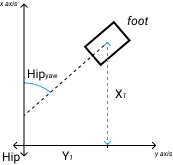
\includegraphics[scale=1.5]{imagens/svg/inverse-kinematics-upperview}
	\caption{Diagrama da visão superior da estrutura de Arash que representa da equação~\ref{eq:ik:upper:hip:yaw} até~\ref{eq:ik:upper:z:2}}
	\caption*{\cite{karimionline}}
	\label{fig:ik:upperview}
\end{figure}

\begin{align}
	P[Hip_{yaw}] &= R_{yaw}                             \label{eq:ik:upper:hip:yaw}  \\
	         X_2 &= T_x cos(R_{yaw}) + T_y sin(R_{yaw})  \label{eq:ik:upper:x:2}      \\
	         Y_2 &= -T_x sin(R_{yaw}) + T_ycos(R_{yaw})   \label{eq:ik:upper:y:2}      \\
	         Z_2 &= T_z                                    \label{eq:ik:upper:z:2}
\end{align}

Seguindo o processo de parametrização dos ângulos das juntas, observa-se na figura~\ref{fig:ik:frontalview} a visão frontal de Arash provendo uma visualização geométrica das equações~\ref{eq:ik:p:hip:roll} até \ref{eq:ik:z:3}.

\begin{figure}[htb]
	\centering
	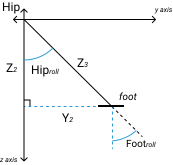
\includegraphics[scale=1.5]{imagens/svg/inverse-kinematics-frontalview}
	\caption{Diagrama da visão frontal de Arash que representa da equação~\ref{eq:ik:p:hip:roll} até~\ref{eq:ik:z:3}}
	\caption*{\cite{karimionline}}
	\label{fig:ik:frontalview}
\end{figure}

\begin{align}
	 P[Hip_{roll}] &= atan\bigg(\dfrac{Y_2}{Z_2}\bigg)                    \label{eq:ik:p:hip:roll}     \\
	P[Foot_{roll}] &= -P[Hip_{roll}] + R_{roll}                            \label{eq:ik:p:foot:roll}    \\
			   X_3 &= X_2                                                   \label{eq:ik:x:3}            \\
			   Y_3 &= Y_2                                                    \label{eq:ik:y:3}            \\
	           Z_3 &= \sqrt{Y_2^{\hspace{1mm}2} + {Z_2}^{\hspace{1mm}2}}      \label{eq:ik:z:3}
\end{align}

Seguindo o processo de parametrização dos ângulos das juntas, observa-se na figura~\ref{fig:ik:frontalview} a visão frontal de Arash provendo uma visualização geométrica das equações~\ref{eq:ik:p:hip:roll} até \ref{eq:ik:z:3}.

\begin{figure}[htb]
	\centering
	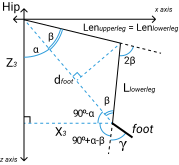
\includegraphics[scale=1.5]{imagens/svg/inverse-kinematics-sideview}
	\caption{Diagrama da visão lateral de Arash que representa da equação~\ref{eq:ik:p:hip:roll} até~\ref{eq:ik:z:3}}
	\caption*{\cite{karimionline}}
	\label{fig:ik:sideview}
\end{figure}

\begin{align}
	       d_{foot} &= \sqrt{Z_3^{\hspace{1mm}2} + X_3^{\hspace{1mm}2}}     \label{eq:ik:d:foot}        \\
	         \alpha &= atan\bigg(\dfrac{X_3}{Z_3}\bigg)                      \label{eq:ik:alpha}         \\
	          \beta &= acos\bigg(\dfrac{d_{foot}}{2 \times Leg_{len}}\bigg)   \label{eq:ik:beta}          \\
	 P[Hip_{pitch}] &= \alpha + \beta                                          \label{eq:ik:p:hip:pitch}   \\
	        P[Knee] &= -2 \beta                                                 \label{eq:ik:p:knee}        \\
	P[Foot_{pitch}] &= \gamma = -\alpha + \beta + R_{pitch}                      \label{eq:ik:p:foot:pitch}
\end{align}

Adicionalmente, em cada junta, é somado um parâmetro de deslocamento -- não incluso nas equações --, também conhecido como \textit{offset}, para compensar possíveis erros provenientes de desalinhamentos no momento de montagem do robô, ou folgas nas engrenagens dos atuadores.

Finalmente, com as equações definidas o \textit{walking gait}, com o auxílio dos componentes de orientação e \textit{proxy}, é apto a fazer os cálculos necessários para determinar os movimentos de caminhada.